%% REFERENCE DRAFT, rewritten 8 Nov 2026 from the user's main.tex (their text up to Allen-Cahn) on their plan: main text
%% compares the mixture, Fourier and neural kernels with a global MLP and a window CNN; the ablations are in the
%% appendix. Read draft2.pdf, or set Menu -> Main document -> draft2.tex in Overleaf. main.tex is the user's paper and is
%% not touched by this file. Figures specific to this draft live in figures/draft/ and are found first.
%% Every number carries a "% src:" comment naming where it was read.
\documentclass{article}
%% Shared by main.tex (the paper you write) and draft.tex (the reference draft).
%% Format: the ICML 2026 kit, two columns, Times text and Computer Modern math. Page geometry, fonts and spacing
%% come from the kit and are never changed here. The kit is the provisional choice until the venue is decided:
%% for a journal (e.g. PRX Intelligence, revtex two-column), only this file and the \twocolumn[...] block in the
%% two main files change.

\usepackage{microtype}
\usepackage{graphicx}
\usepackage{booktabs}
\usepackage{xcolor}
\usepackage{hyperref}
\usepackage{tikz}
\usetikzlibrary{arrows.meta,calc,positioning}
\newcommand{\theHalgorithm}{\arabic{algorithm}}

% preprint: author names shown, footer "Preprint. <date>" (arXiv first, venue later).
% Anonymous submission: \usepackage{icml2026}.  Camera-ready: \usepackage[accepted]{icml2026}.
\usepackage[preprint]{icml2026}

\usepackage{amsmath}
\usepackage{amssymb}
\usepackage{mathtools}
\usepackage[capitalize,noabbrev]{cleveref}

\graphicspath{{figures/}}

%% ---------------------------------------------------------------- figures
%% Every plot is drawn at its printed size: 3.25 in for one column, 6.75 in for the full width (figure*).
%% Include them WITHOUT a width, so that the axis labels stay at the body's 10 pt:
%%     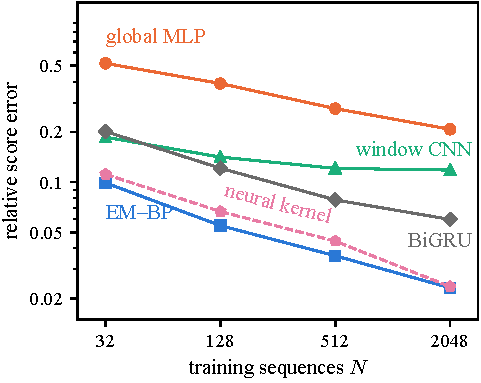
\includegraphics{fig_value_of_structure}
%% The plots and their style (box on all four sides, no grid, minor ticks, log scales, markers for measurements and
%% lines for closed forms) are made by tools/paper_figs/make_paper_figures.py in the research repository; see README.md.
%% The two diagrams are TikZ, \input from figures/*.tikz, so they use the body font and can be edited here.

%% ---------------------------------------------------------------- notation
\newcommand{\E}{\mathbb{E}}
\newcommand{\Normal}{\mathcal{N}}
\newcommand{\Kt}{K_\theta}
\newcommand{\dd}{\mathrm{d}}
\newcommand{\Dt}{\Delta_t}
\newcommand{\Ng}{N_g}

%% ---------------------------------------------------------------- writing aids
%% \note{...}    grey guidance text: what goes here, what Jerome asked for. Hide them all with \shownotesfalse.
%% \pending{...} a result that is not in yet (a run still on the cluster). Shown in orange so none is forgotten.
\newif\ifshownotes \shownotestrue
\definecolor{notegrey}{gray}{0.45}
\definecolor{pendingorange}{HTML}{C0501F}
\newcommand{\note}[1]{\ifshownotes{\color{notegrey}\itshape [#1]}\fi}
\newcommand{\pending}[1]{{\color{pendingorange}[pending: #1]}}

\graphicspath{{figures/draft/}{figures/}}

\icmltitlerunning{Learning Scores for Markov Sequences in Generative Diffusion}

\begin{document}

\twocolumn[
\icmltitle{Learning Scores for Markov Sequences in Generative Diffusion}

\begin{icmlauthorlist}
  \icmlauthor{Giovanni Mantovani}{boc}
  \icmlauthor{J\'er\^ome Garnier-Brun}{boc}
  \icmlauthor{Marc M\'ezard}{boc}
\end{icmlauthorlist}
\icmlaffiliation{boc}{Department of Computing Sciences, Bocconi University, Milan, Italy}
\icmlcorrespondingauthor{Giovanni Mantovani}{giovanni-mantovani@studbocconi.it}
\icmlkeywords{diffusion models, belief propagation, expectation maximisation, Markov chains}
\vskip 0.3in
]

\printAffiliationsAndNotice{}

\begin{abstract}
Diffusion models learn to denoise data at every noise level, and the object they need is the score, an affine function
of the posterior mean. We ask how to compute it for Markov sequences. In the Gaussian case the score is linear and set
by a precision matrix, and we see how noise quickly erases its Markov structure. In the Laplace case the score has no
closed form, but the posterior is a tree, so belief propagation (BP) gives the exact score. Its messages
are probability densities: we discretise them on a grid and test the discretisation against the Gaussian closed form.
When the transition kernel is unknown we learn it, with expectation--maximisation from noisy sequences or with maximum
likelihood from clean ones, and BP turns it into the score at every noise level. The kernel can be a small neural
network. On the Laplace chain, kernels learned this way give scores 2 to 10 times more accurate than a global MLP and a
window CNN trained by denoising score matching, with far fewer parameter updates. On the stochastic Allen--Cahn field,
where the shape of the transition law changes with the state, a Gaussian-mixture kernel is no better than a linear
denoiser, while the neural kernel stays accurate.
% src: Laplace, per-seed mean ratios over N = 32..2048, 16 seeds, paired (E02a, E56, E03): window CNN / kernel
% 1.84-5.58, global MLP / kernel 5.18-9.85. Allen-Cahn Theta = 0.3, N = 2048: E33 mixture 0.2705 vs linear 0.2692;
% E55 neural kernel 0.0328, 2.6 times below the window CNN (E58).

\end{abstract}

\section{Introduction}
\label{sec:intro}

Diffusion models are inspired by nonequilibrium thermodynamics \cite{sohl2015deep} and are now the standard generative
models for pictures \cite{rombach2022latent,betker2023dalle3}, videos \cite{veo3}, 3D protein structures
\cite{abramson2024alphafold3} and many other kinds of data. They reverse a stochastic differential equation
\cite{anderson1982reverse,ho2020denoising,song2021scorebased} using the score
$\mathbf{s}_t(\mathbf{x})=\nabla_{\mathbf{x}}\log p_t(\mathbf{x})$, which can be rewritten as a posterior mean
\cite{robbins1956empirical,vincent2011connection,efron2011tweedie}. Much has been learned about how these models work.
They go through distinct dynamical regimes \cite{biroli2023generative,biroli2024dynamical,achilli2026speciation}, which
become a cascade of speciations when the data have long-range correlations \cite{garnierbrun2026foam}. They generalise
instead of memorising for reasons that are now partly understood
\cite{kadkhodaie2024generalization,achilli2025memorization,bonnaire2025memorize}, and their generalisation can be biased
\cite{garnierbrun2026biased}.

Here we work with Markov sequences, such as time series or one-dimensional physical fields with nearest-neighbour
interactions. We want to understand what a denoiser gains from knowing that the data are Markov, and how to use it. We
start from the Gaussian case, where the score has a linear closed form set by a precision matrix (\cref{sec:gaussian}).
The simplest case where the score is not linear is the Laplace chain, and there we compute the exact score with message
passing \cite{pearl1988probabilistic,mezard2002analytic,mezard2003passing,mezard2009information}
(\cref{sec:tree,sec:grid}). Finally, we learn the kernel (\cref{sec:laplace}) and test the method on the stochastic
Allen--Cahn field \cite{allen1979microscopic} (\cref{sec:allen-cahn}).

Our main contributions are:
\begin{itemize}
\item For any first-order Markov chain, belief propagation gives the exact score, because a Markov chain observed through
  independent noise is a tree (\cref{sec:tree}).
\item When the kernel is unknown, we learn it with expectation--maximisation if we only see noisy sequences, or with
  maximum likelihood if we have the clean ones. The kernel can be a small neural network, and BP turns it into the score.
  In our experiments this is more accurate than denoising score matching with a global MLP or a window CNN, and it needs
  far fewer parameter updates (\cref{sec:laplace}).
\item We discretise the messages on a grid and test the discretisation against the Gaussian closed form. On the Laplace
  chain the grid error is four orders of magnitude below the error of a Gaussian approximation (\cref{sec:grid}).
\item We go beyond the Gaussian and the Laplace chains to a physical field, the stochastic Allen--Cahn equation, where the
  shape of the transition law changes with the state (\cref{sec:allen-cahn}).
\end{itemize}

\section{Setting}
\label{sec:setting}

\paragraph{Clean data.}
We consider real-valued sequences
$\mathbf{a}=(a_1,\ldots,a_L)\in\mathbb{R}^L$
generated by a first-order Markov chain. The Markov property
states that the conditional distribution of the next state
depends only on the current state:
\begin{equation}
p(a_{k+1}\mid a_1,\ldots,a_k)
=
p(a_{k+1}\mid a_k).
\end{equation}
Consequently, the joint distribution factorises as
\begin{equation}
p_0(\mathbf{a})
=
\mu(a_1)
\prod_{k=1}^{L-1}
K(a_{k+1}\mid a_k),
\label{eq:markov_prior}
\end{equation}
where $\mu$ is the initial-state distribution and
$K(a'\mid a)$ is the transition kernel, satisfying
\begin{equation}
K(a'\mid a)\geq 0,
\qquad
\int_{\mathbb{R}} K(a'\mid a)\,da'=1.
\end{equation}
We assume a stationary chain with unit variance, so that
the same transition kernel is used at every position. Nothing
below requires it: with a different kernel $K_k$ at each
position, every formula holds with $K$ replaced by $K_k$.

\paragraph{Ornstein--Uhlenbeck corruption.}
We corrupt each coordinate independently through a
variance-preserving Ornstein--Uhlenbeck (OU) process
\cite{song2021scorebased}:
\begin{equation}
dx_k(t)=-x_k(t)\,dt+\sqrt{2}\,dW_k(t),
\end{equation}
where $W_k(t)$ are independent standard Wiener processes.
Starting from $x_k(0)=a_k$, its solution at time $t$ is
\begin{equation}
x_k=e^{-t}a_k+\sqrt{\Delta_t}\,\xi_k,
\qquad
\xi_k\sim\mathcal{N}(0,1),
\label{eq:ou_corruption}
\end{equation}
with $\Delta_t=1-e^{-2t}$.
The corresponding conditional density factorises over
coordinates:
\begin{equation}
p_t(\mathbf{x}\mid\mathbf{a})
=
\prod_{k=1}^{L}
\ell_t(x_k\mid a_k),
\label{eq:ou_likelihood}
\end{equation}
with $\ell_t(x_k\mid a_k)=\mathcal{N}(x_k;e^{-t}a_k,\Delta_t)$.

\paragraph{Posterior distribution.}
Combining the Markov prior with the independent observation
likelihood gives
\begin{equation}
p_t(\mathbf{a}\mid\mathbf{x})
\propto
\mu(a_1)
\prod_{k=1}^{L-1}K(a_{k+1}\mid a_k)
\prod_{k=1}^{L}\ell_t(x_k\mid a_k).
\label{eq:posterior_chain}
\end{equation}

Moreover, the noisy score can be expressed in terms of the posterior mean
(Tweedie's formula \cite{robbins1956empirical,efron2011tweedie}):
\begin{equation}
    \mathbf S_t(\mathbf x)
    := \nabla_{\mathbf x}\log p_t(\mathbf x)
    =
    \frac{e^{-t}\mathbb E[\mathbf a\mid\mathbf x]-\mathbf x}
         {\Delta_t}.
    \label{eq:tweedie}
\end{equation}

\section{The Gaussian chain: diffusion breaks locality}
\label{sec:gaussian}

\begin{figure*}[t]
  \centering
  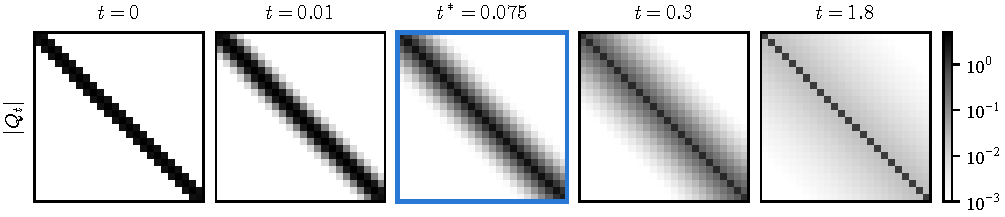
\includegraphics{fig_locality}
  \caption{Noise makes the score non-local. Magnitude of the matrix $\mathbf Q_t$ in the score
  $\mathbf S_t(\mathbf x)=-\mathbf Q_t\mathbf x$ of the Gaussian chain ($\alpha=0.85$, $L=24$) at five noise levels, on
  a log colour scale. At $t=0$ it is tridiagonal; at large $t$ it tends to the identity; in between, at
  $t^{*}\simeq0.075$ (framed), it is furthest from tridiagonal.}
  \label{fig:locality}
  % src: closed form, tools/paper_figs/make_paper_figures.py::fig_locality (t* = 0.0753 printed by the generator)
\end{figure*}

As an exactly solvable baseline, consider the stationary Gaussian chain
\begin{equation}
    a_{k+1}=\alpha a_k+\eta_k,
    \qquad \eta_k\sim\mathcal N(0,1-\alpha^2),
\end{equation}
where $\alpha\in(-1,1)$ sets the correlation between consecutive sites and the noise variance $1-\alpha^2$ keeps the
chain stationary with unit variance. Its joint distribution is Gaussian,
$p_0(\mathbf a)=\mathcal N(\mathbf 0,\boldsymbol\Sigma_0)$ with $(\boldsymbol\Sigma_0)_{ij}=\alpha^{|i-j|}$, and its
precision matrix $\mathbf Q_0=\boldsymbol\Sigma_0^{-1}$ is tridiagonal: this is the Markov property, written as a
statement about the score.

Under the noise of \cref{eq:ou_corruption} the data stay Gaussian,
\begin{equation}
    p_t(\mathbf x)=\mathcal N(\mathbf 0,\boldsymbol\Sigma_t),
    \qquad
    \boldsymbol\Sigma_t
    =e^{-2t}\boldsymbol\Sigma_0+\Delta_t\mathbf I,
\end{equation}
so the score is exactly linear:
\begin{equation}
    \mathbf S_t(\mathbf x)
    =-\mathbf Q_t\mathbf x,
    \qquad \mathbf Q_t=\boldsymbol\Sigma_t^{-1}.
\end{equation}
While $\mathbf Q_0$ is tridiagonal, $\mathbf Q_t$ is dense for $t>0$ (\cref{fig:locality}). Diffusion turns a locally
structured chain into a distribution whose score is not local, even though the distribution stays Gaussian. The effect
is strongest at an intermediate noise level, $t^{*}\simeq0.075$ for $\alpha=0.85$, and fades at large $t$, where the
noise dominates.
% src: t* = 0.0753, fig_locality / fig_locality_curve

So locality cannot simply be imposed on the denoiser. A denoiser that only looks at the two neighbours of each site
has a relative score error of $0.20$ even with unlimited data. The structure survives elsewhere: the posterior
$p_t(\mathbf a\mid\mathbf x)$ of \cref{eq:posterior_chain} is still a chain, because the noise adds one factor per site
and no new link. For the Gaussian chain, inference along this chain returns $-\mathbf Q_t\mathbf x$ exactly in $O(L)$
operations, without ever forming $\mathbf Q_t$. The next sections do the same for any kernel.
% src: thesis tools/fig_ch10.py::windowed_oracle([1]) = 0.2023 (alpha=0.85, L=32, twelve levels)

\section{A noisy Markov chain is a tree}
\label{sec:tree}

\begin{figure}[t]
  \centering
  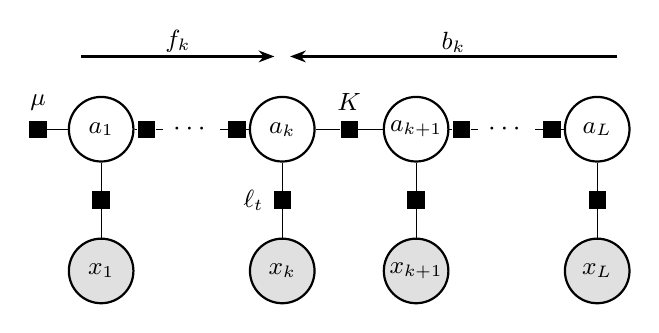
\begin{tikzpicture}[
    var/.style={circle,draw,thick,minimum size=8.2mm,inner sep=0pt,font=\small},
    obs/.style={circle,draw,thick,fill=black!12,minimum size=8.2mm,inner sep=0pt,font=\small},
    fac/.style={rectangle,fill=black,minimum size=2.2mm,inner sep=0pt},
    lab/.style={font=\small,inner sep=1pt},
    msg/.style={-{Stealth[length=2mm]},thick}]
  \node[var] (a1) at (0,0) {$a_1$};
  \node (d1) at (1.15,0) {$\cdots$};
  \node[var] (ak) at (2.3,0) {$a_k$};
  \node[var] (ak1) at (4.0,0) {$a_{k+1}$};
  \node (d2) at (5.15,0) {$\cdots$};
  \node[var] (aL) at (6.3,0) {$a_L$};
  \node[fac] (m0) at (-0.8,0) {};
  \draw (m0) -- (a1);
  \node[lab,above=0.8mm of m0] {$\mu$};
  \foreach \u/\v/\n in {a1/d1/ka,d1/ak/kb,ak/ak1/kc,ak1/d2/kd,d2/aL/ke} {
    \node[fac] (\n) at ($(\u)!0.5!(\v)$) {};
    \draw (\u) -- (\n) -- (\v);
  }
  \node[lab,above=0.8mm of kc] {$K$};
  \foreach \i/\n in {a1/1,ak/k,ak1/{k+1},aL/L} {
    \node[fac] (o\i) at ($(\i)+(0,-0.9)$) {};
    \node[obs] (x\i) at ($(\i)+(0,-1.8)$) {$x_{\n}$};
    \draw (\i) -- (o\i) -- (x\i);
  }
  \node[lab,left=0.8mm of oak] {$\ell_t$};
  \draw[msg] ($(a1.north)+(-0.25,0.5)$) -- node[lab,above]{$f_k$} ($(ak.north)+(-0.1,0.5)$);
  \draw[msg] ($(aL.north)+(0.25,0.5)$) -- node[lab,above]{$b_k$} ($(ak.north)+(0.1,0.5)$);
\end{tikzpicture}

  \caption{Factor graph of the posterior $p_t(\mathbf a\mid\mathbf x)$ of \cref{eq:posterior_chain}. White circles are
  the clean values $a_k$, grey circles the noisy observations $x_k$, which are known. Black squares are the factors: the
  law $\mu$ of the first site, the kernel $K(a_{k+1}\mid a_k)$ between neighbours and the noise term
  $\ell_t(x_k\mid a_k)$ at each site. There is no loop, so belief propagation is exact. The forward message $f_k$ carries
  what $x_1,\ldots,x_k$ say about $a_k$, the backward message $b_k$ what $x_{k+1},\ldots,x_L$ say about it, and the
  posterior of $a_k$ is proportional to $f_k(a_k)\,b_k(a_k)$.}
  \label{fig:factor-graph}
\end{figure}

\paragraph{Beyond Gaussianity.}
The Gaussian chain is exactly solvable and linear. We now take a controlled non-Gaussian step, the Laplace chain
\begin{equation}
    a_{k+1}=\alpha a_k+\varepsilon_k,
    \qquad
    \varepsilon_k\sim\operatorname{Laplace}(0,b),
    \label{eq:laplace_chain}
\end{equation}
with $2b^2=1-\alpha^2$. The noise has the same variance as in the Gaussian chain, so the two chains have the same
covariance. But the Laplace noise has a sharp peak and heavier tails, and the score is no longer linear in $\mathbf x$.
At small noise it saturates: a large jump in the data is believed, because the Laplace chain does make jumps, and only
a bounded part of it is put down to the diffusion noise (\cref{app:gaussian-laplace}).

\paragraph{The posterior factor graph.}
The first-order Markov structure survives the noise. Combining the kernel with the independent noise terms gives
\cref{eq:posterior_chain}, whose factor graph is a chain with one extra factor on each site (\cref{fig:factor-graph}).
Since the noise acts on each site separately, conditioning on the observations adds no edge. The posterior is still
connected and has no loop: it is a tree, where the cavity method and belief propagation are exact
\cite{mezard2001bethe,mezard2006reconstruction,mezard2009information}.

\paragraph{Exact inference by belief propagation.}
On a tree, the sum--product algorithm gives the exact marginals with one forward and one backward pass
\cite{pearl1988probabilistic,kschischang2001factor,yedidia2003understanding}. With forward messages $f_k$ and backward
messages $b_k$, the recursions are
\begin{align}
    f_1(a_1)
    &=\mu(a_1)\ell_t(x_1\mid a_1),\nonumber\\
    f_{k+1}(a_{k+1})
    &=\ell_t(x_{k+1}\mid a_{k+1})\nonumber\\
    &\qquad\times\int K(a_{k+1}\mid a_k)f_k(a_k)\,da_k,\nonumber\\
    b_L(a_L)&=1,\nonumber\\
    b_k(a_k)
    &=\int K(a_{k+1}\mid a_k)
      \ell_t(x_{k+1}\mid a_{k+1})\nonumber\\
    &\qquad\times b_{k+1}(a_{k+1})\,da_{k+1}.
    \label{eq:bp}
\end{align}
The posterior of one site is then
\begin{equation}
    p(a_k\mid\mathbf x)
    \propto f_k(a_k)b_k(a_k),
\end{equation}
and its mean gives the score through \cref{eq:tweedie}:
\begin{equation}
    S_{t,k}(\mathbf x)=\frac{e^{-t}}{\Delta_t}\,
    \frac{\int a\,f_k(a)b_k(a)\,da}{\int f_k(a)b_k(a)\,da}-\frac{x_k}{\Delta_t}.
\end{equation}

So, for any known first-order kernel, two sweeps of messages give the exact joint score, with no assumption of
Gaussianity or linearity. The noise level only enters through $\ell_t$, so one kernel gives the score at every $t$.
The same exact inference on a tree is at the heart of the hierarchical models of \cite{garnierbrun2024transformers},
where transformers trained on such data learn to approximate BP; a Markov chain is the simplest tree.

\section{Messages are probability densities}
\label{sec:grid}

Unlike in discrete-state models, each latent variable here is a real number, $a_k\in\mathbb R$. A BP message is
therefore a non-negative function of a continuous variable, not a finite vector, and the message updates involve
integrals over $\mathbb R$ that have no closed form for a non-Gaussian kernel.

We compute these integrals numerically on a uniform grid
\begin{equation}
    g_i=-A+ih,\quad i=0,\ldots,N_g-1,\quad h=2A/(N_g-1),
\end{equation}
on $[-A,A]$, with trapezoidal weights $w_i$; we use $A=8$ and $N_g=401$, so $h=0.04$. The kernel and the noise terms
become a matrix and vectors,
\begin{equation}
    K_{ij}=K(g_i\mid g_j),
    \qquad
    (\ell_k)_i=\ell_t(x_k\mid g_i),
\end{equation}
and each integral in the recursions becomes a weighted matrix--vector product:
\begin{align}
    f_{k+1}
    &\propto
    \ell_{k+1}\odot K(w\odot f_k),\\
    b_k
    &\propto
    K^\top(w\odot\ell_{k+1}\odot b_{k+1}),
\end{align}
where $\odot$ is the elementwise product and $w=(w_0,\ldots,w_{N_g-1})^\top$. The messages are normalised after each
update for numerical stability, and the posterior mean is
\begin{equation}
    \widehat m_k
    =
    \frac{\sum_i w_i g_i(f_k)_i(b_k)_i}
         {\sum_i w_i(f_k)_i(b_k)_i},
\end{equation}
which goes into Tweedie's formula to give the score.

A sequence costs $O(LN_g^2)$ operations. The grid introduces a discretisation error, which we control by refining the
grid and enlarging the domain, and which we test against the Gaussian chain, where the exact score is known. There grid
BP matches $-\mathbf Q_t\mathbf x$ to double-precision round-off for $t\geq0.05$, our smallest noise level. On the
Laplace chain, going from 401 to 801 points changes the score by about $10^{-5}$ in relative terms (\cref{app:bp}).
% src: fig_grid_gaussian (exp_01/grid_sweep_M.csv); figs_v2._closure_sweep, grid 401 vs 801 median 1.10e-5 at t=0.05

\begin{figure}[t]
  \centering
  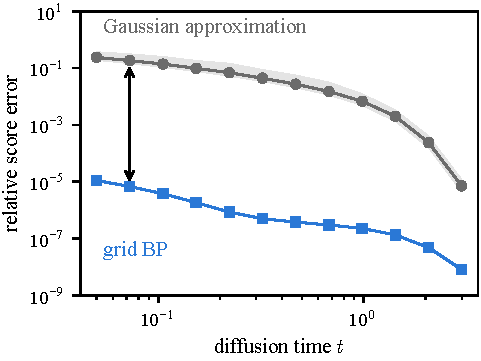
\includegraphics{fig_closure}
  \caption{What a Gaussian approximation costs on the Laplace chain ($\alpha=0.85$, $L=32$, true kernel). Relative
  score error against grid BP on 801 points, at the twelve noise levels used in the experiments; median over 2{,}000
  sequences, with the 10--90\% range shaded. Gaussian approximation: Gaussian messages, which give the score of the
  Gaussian chain with the same covariance. Grid BP: the 401-point grid used in every experiment. Details in
  \cref{app:measures}.}
  \label{fig:grid-vs-gaussian}
  % src: tools/paper_figs/figs_v2.py::_closure_sweep (reports/paper-figures/data/closure_sweep_2000.csv)
\end{figure}

\paragraph{Why not a Gaussian approximation?}
A natural alternative is to approximate each message by a Gaussian, keeping only its mean and variance. This is exact
for the Gaussian chain, because Gaussian kernels and noise terms stay Gaussian under the products and integrals of BP.
It is not exact for the Laplace chain: Gaussian messages throw away what is non-Gaussian and give back the score of the
Gaussian chain with the same covariance, which is linear in $\mathbf x$ and cannot see the peak of the Laplace law.

This matters most at small noise, where the Laplace score saturates. \Cref{fig:grid-vs-gaussian} shows the cost: at
$t=0.05$ the Gaussian approximation has a median relative error of $0.24$, against $10^{-5}$ for grid BP. The gap closes
as $t$ grows, because both scores become linear.
% src: closure_sweep_2000.csv: t=0.05 lin_med 0.2387, grid_med 1.10e-5

This is also different from approximate message passing (AMP) and Thouless--Anderson--Palmer (TAP) methods
\cite{thouless1977solution,mezard1986sk,mezard1987spin,kabashima2003cdma,donoho2009message,krzakala2012statistical,bolthausen2014iterative}.
Those are built for dense, high-dimensional systems, where many weak interactions justify Gaussian messages with an
Onsager correction \cite{zdeborova2016statistical,mezard2017meanfield,lauditi2023sparse}. Our factor graph is a chain,
where each variable has two neighbours: ordinary belief propagation is already exact, so we discretise the messages
rather than approximate them.

\section{Learning the kernel}
\label{sec:laplace}

In practice the kernel is unknown and has to be learned from data. We work on the Laplace chain, where the exact score
is known and not linear, and compare learning the kernel with training neural denoisers by denoising score matching.

\subsection{Expectation--maximisation through BP}
\label{sec:em}

\begin{figure}[t]
  \centering
  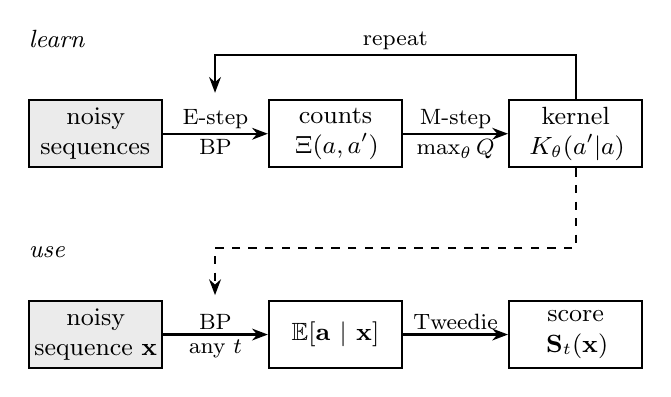
\begin{tikzpicture}[
    box/.style={draw,thick,align=center,font=\small,minimum height=8.5mm,inner sep=2pt,text width=1.55cm},
    data/.style={box,fill=black!8},
    arr/.style={-{Stealth[length=2mm]},thick},
    lab/.style={font=\footnotesize,align=center,inner sep=1.5pt},
    stage/.style={font=\small\itshape,anchor=west,inner sep=0pt}]
  \node[stage] at (-0.85,1.2) {learn};
  \node[data] (x) at (0,0) {noisy\\ sequences};
  \node[box] (xi) at (3.05,0) {counts\\ $\Xi(a,a')$};
  \node[box] (k) at (6.1,0) {kernel\\ $K_\theta(a'|a)$};
  \draw[arr] (x) -- node[lab,above]{E-step} node[lab,below]{BP} (xi);
  \draw[arr] (xi) -- node[lab,above]{M-step} node[lab,below]{$\max_\theta Q$} (k);
  \draw[arr] (k.north) |- node[lab,above,pos=0.75]{repeat} (1.52,1.0) -- (1.52,0.52);
  \node[stage] at (-0.85,-1.5) {use};
  \node[data] (y) at (0,-2.55) {noisy\\ sequence $\mathbf{x}$};
  \node[box] (m) at (3.05,-2.55) {$\mathbb{E}[\mathbf{a}\mid\mathbf{x}]$};
  \node[box] (s) at (6.1,-2.55) {score\\ $\mathbf{S}_t(\mathbf{x})$};
  \draw[arr] (y) -- node[lab,above]{BP} node[lab,below]{any $t$} (m);
  \draw[arr] (m) -- node[lab,above]{Tweedie} (s);
  \draw[thick,dashed,-{Stealth[length=2mm]}] (k.south) |- (1.52,-1.45) -- (1.52,-2.05);
\end{tikzpicture}

  \caption{Learning and using the kernel. Learn: BP with the current kernel gives the posterior of every pair of
  neighbouring sites, summed into the expected transition counts $\Xi$ (E-step); the kernel is refitted to these
  counts (M-step); repeat. Use: BP with the learned kernel gives $\mathbb E[\mathbf a\mid\mathbf x]$, and so the score,
  at any noise level. BP enters the learning only through $\Xi$, so nothing is differentiated through BP.}
  \label{fig:em-loop}
\end{figure}

Let $K_\theta$ be a family of kernels and $\mathbf{x}^{(1)},\ldots,\mathbf{x}^{(N)}$ noisy training sequences, each
observed at a noise level $t_d$. The clean sequences are latent variables, and the likelihood of the data is
\begin{equation}
    p_\theta(\mathbf{x}^{(d)})
    =
    \int
    p_\theta(\mathbf{a})
    p_{t_d}(\mathbf{x}^{(d)}\mid\mathbf{a})
    \,d\mathbf{a}.
\end{equation}
This integral has no closed form, but BP computes it on the chain, from the normalising constants of the forward
messages (\cref{app:bp}).

We maximise it with expectation--maximisation (EM) \cite{dempster1977maximum}, as in the Baum--Welch algorithm for
hidden Markov models \cite{baum1970,rabiner1989tutorial}: the clean sequence is the hidden chain and the diffusion noise
is the emission (\cref{fig:em-loop}). The E-step uses the current parameters $\theta_{\mathrm{old}}$ to infer the
posterior of each pair of neighbouring sites,
\begin{equation}
    \xi_k^{(d)}(a,a')
    =
    p_{\theta_{\mathrm{old}}}
    \left(
        a_k=a,\,
        a_{k+1}=a'
        \mid \mathbf{x}^{(d)}
    \right),
\end{equation}
which the forward and backward messages give directly:
\begin{equation}
    \xi_k^{(d)}(a,a')
    \propto
    f_k(a)\,
    K_{\theta_{\mathrm{old}}}(a'\mid a)\,
    \ell_{t_d}(x_{k+1}^{(d)}\mid a')\,
    b_{k+1}(a').
    \label{eq:pairwise-posterior}
\end{equation}
Summing over sequences and links gives the expected transition counts
\begin{equation}
    \Xi(a,a')
    =
    \sum_{d=1}^{N}
    \sum_{k=1}^{L-1}
    \xi_k^{(d)}(a,a'),
\end{equation}
the expected number of transitions from $a$ to $a'$ in the clean data. The M-step then maximises
\begin{equation}
    Q(\theta\mid\theta_{\mathrm{old}})
    =
    \iint
    \Xi(a,a')\,
    \log K_\theta(a'\mid a)
    \,da\,da'
    \label{eq:em-objective}
\end{equation}
over $\theta$. With clean sequences nothing is hidden: $\Xi$ is just the histogram of the observed transitions and the
M-step is ordinary maximum likelihood. With noisy sequences the counts are soft, and BP provides them.

Why does this work? By Fisher's identity \cite{louis1982,cappe2005}, the gradient of $Q$ at $\theta_{\mathrm{old}}$ is
the gradient of the log-likelihood,
\begin{equation}
    \left.
    \nabla_\theta Q(\theta\mid\theta_{\mathrm{old}})
    \right|_{\theta=\theta_{\mathrm{old}}}
    =
    \nabla_\theta
    \log p_\theta(\mathbf{x})
    \big|_{\theta=\theta_{\mathrm{old}}},
\end{equation}
so each M-step moves uphill and the likelihood never decreases \cite{dempster1977maximum,wu1983}. Two practical
consequences follow. BP enters the M-step only through $\Xi$, which stays fixed while $\theta$ moves, so there is no
need to differentiate through the messages: the gradient only goes through the kernel and its normalisation. And the
noise level appears only in the E-step, so the kernel is learned once and then gives the score at any noise level.

\subsection{Kernel families}
\label{sec:kernel-families}

We first use families with the shift structure $a_{k+1}=\alpha a_k+\varepsilon_k$, where the noise $\varepsilon_k$ does
not depend on $a_k$. One option is a mixture of $C=8$ Gaussians for the noise,
\begin{equation}
    K_\theta(a'\mid a)
    =
    \sum_{c=1}^{C}
    \pi_c\,
    \mathcal{N}
    \left(
        a'-\alpha a;\nu_c,s_c^2
    \right),
\end{equation}
with weights $\pi_c$ summing to one. It has 25 parameters and an almost closed-form M-step, and it learns $\alpha$
quickly (to $0.1\%$ from 512 sequences), but it can only approximate the peak of the Laplace law by stacking Gaussians.
A second option writes the logarithm of the noise density as a truncated Fourier series, again with 25 parameters; this
keeps the kernel positive and makes the M-step concave. Other bases behave the same way (\cref{app:families}).
% src: thesis exp_18: alpha within 0.1% from N=512 (2.4% at 128)

Both families assume the shift structure. We therefore also use a kernel that assumes nothing beyond the Markov
property, a neural energy kernel, which we simply call the neural kernel:
\begin{equation}
    K_\theta(a'\mid a)
    =
    \frac{
        \exp[-E_\theta(a,a')]
    }{
        Z_\theta(a)
    },
    \label{eq:neural-kernel}
\end{equation}
with $Z_\theta(a)=\int\exp[-E_\theta(a,u)]\,du$ computed on the grid. $E_\theta$ is a small network with two hidden
layers of 16 units, 337 parameters in all, and the normalisation makes $K_\theta$ a valid transition density for any
weights.

With noisy sequences the neural kernel is trained by the same EM: BP gives $\Xi$ in the E-step, and the M-step takes
ten Adam steps \cite{kingma2015adam} on \cref{eq:em-objective}, differentiating only through the kernel. With clean
sequences it can instead be fitted by maximising the likelihood of the observed transitions,
\begin{equation}
    \mathcal{L}(\theta)
    =
    \sum_{d=1}^{N}
    \sum_{k=1}^{L-1}
    \log K_\theta
    \left(
        a_{k+1}^{(d)}
        \mid a_k^{(d)}
    \right),
    \label{eq:neural-clean-ml}
\end{equation}
with no E-step at all. The same kernel can therefore be learned from noisy sequences by EM or from clean ones by
maximum likelihood.

\subsection{Against neural denoisers}
\label{sec:neural-denoisers}

\begin{figure}[t]
  \centering
  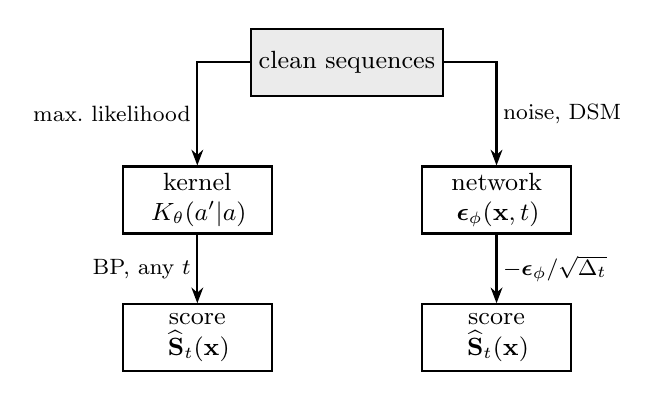
\begin{tikzpicture}[
    box/.style={draw,thick,align=center,font=\small,minimum height=8.5mm,inner sep=2pt,text width=1.75cm},
    data/.style={box,fill=black!8,text width=2.3cm},
    arr/.style={-{Stealth[length=2mm]},thick},
    lab/.style={font=\footnotesize,align=center,inner sep=2pt}]
  \node[data] (a) at (0,0) {clean sequences};
  \node[box] (k) at (-1.9,-1.75) {kernel\\ $K_\theta(a'|a)$};
  \node[box] (n) at (1.9,-1.75) {network\\ $\boldsymbol{\epsilon}_\phi(\mathbf{x},t)$};
  \node[box] (s1) at (-1.9,-3.5) {score\\ $\widehat{\mathbf{S}}_t(\mathbf{x})$};
  \node[box] (s2) at (1.9,-3.5) {score\\ $\widehat{\mathbf{S}}_t(\mathbf{x})$};
  \draw[arr] (a.west) -| node[lab,left,pos=0.75]{max.\ likelihood} (k.north);
  \draw[arr] (a.east) -| node[lab,right,pos=0.75]{noise, DSM} (n.north);
  \draw[arr] (k) -- node[lab,left]{BP, any $t$} (s1);
  \draw[arr] (n) -- node[lab,right]{$-\boldsymbol{\epsilon}_\phi/\sqrt{\Delta_t}$} (s2);
\end{tikzpicture}

  \caption{Two ways to learn from the same clean sequences. Left: fit the kernel by maximum likelihood
  (\cref{eq:neural-clean-ml}); BP then gives the score at any noise level. Right: train a network by denoising score
  matching on noisy copies of the sequences (\cref{eq:dsm-objective}); it gives the score at the noise levels it was
  trained on. The kernel is a function of two numbers; the network has to learn the whole map from $(\mathbf x,t)$ to
  the score.}
  \label{fig:routes}
\end{figure}

We compare the learned kernels with neural denoisers trained by denoising score matching (DSM)
\cite{hyvarinen2005estimation,vincent2011connection}. These do not model the transition law; they learn the score
directly from noisy sequences. For a clean sequence $\mathbf a$ the noisy version is
\begin{equation}
    \mathbf{x}
    =
    e^{-t}\mathbf{a}
    +
    \sqrt{\Delta_t}\boldsymbol{\xi},
    \qquad
    \boldsymbol{\xi}
    \sim
    \mathcal{N}(\mathbf{0},\mathbf{I}),
\end{equation}
and a network $\boldsymbol{\epsilon}_\phi(\mathbf{x},t)$ is trained to predict the added noise by minimising
\begin{equation}
    \mathcal{L}_{\mathrm{DSM}}(\phi)
    =
    \mathbb{E}_{\mathbf{a},t,\boldsymbol{\xi}}
    \left[
        \left\|
            \boldsymbol{\xi}
            -
            \boldsymbol{\epsilon}_\phi
            (\mathbf{x},t)
        \right\|^2
    \right],
    \label{eq:dsm-objective}
\end{equation}
which gives the score estimate $\widehat{\mathbf{S}}_t(\mathbf{x})=-\boldsymbol{\epsilon}_\phi(\mathbf{x},t)/\sqrt{\Delta_t}$.

We use a global MLP, which knows nothing about locality, and a window CNN, which only looks at nearby sites (26{,}016
and 5{,}505 parameters). Both are trained on the clean sequences with fresh noise at every step (\cref{fig:routes}),
with hyperparameters chosen on separate seeds (\cref{app:networks}, which also has four other architectures). The
comparison is between two approaches: learning a small transition law and letting BP do the inference, or learning the
whole denoiser from examples. In the first the Markov structure is built into the model; in the second the network has
to find it in the data.
% src: outputs/E03/winners.json, confirm.csv n_params (mlp 26,016; window 5,505)

\subsection{Results on the Laplace chain}
\label{sec:results}

\begin{figure*}[t]
  \centering
  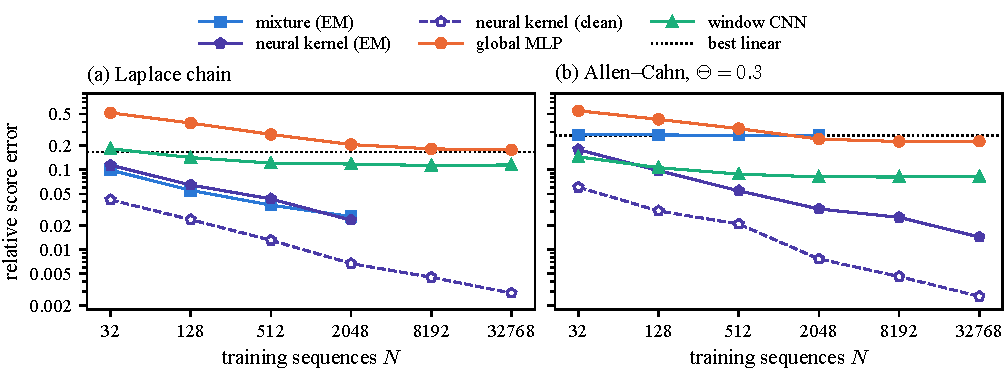
\includegraphics{fig_results}
  \caption{Relative score error against the number of training sequences $N$. (a) Laplace chain, 16 seeds.
  (b) Allen--Cahn field at $\Theta=0.3$ (\cref{sec:allen-cahn}), 8 seeds. Filled markers: kernels learned by EM from
  noisy sequences and used inside BP, the mixture of 8 Gaussians and the neural kernel. Open markers, dashed: the neural
  kernel fitted by maximum likelihood on the clean sequences. Global MLP and window CNN: denoising score matching on the
  clean sequences. Dotted: the best linear denoiser. Medians over seeds; on the Laplace chain the EM runs stop at
  $N=2048$.}
  \label{fig:results}
  % src: tools/paper_figs/figs_v2.py::fig_results. (a) E02a capacity.csv (em_bp, C=8), E56 kernels (energy), E58
  % (energy_h16, mlp, window, lmmse; E58's gate G2 reproduces E03's networks at N <= 2048). (b) E33 via read_e60
  % (em_mixture, raw_risk), E55 kernels (em_energy, selection=risk), E58 (energy_h16, mlp, window, lmmse); seeds 0-7.
\end{figure*}

We use the Laplace chain with $\alpha=0.85$ and $L=32$, and twelve noise levels between $t=0.05$ and $t=3$. Each model
is trained on $N$ sequences, from 32 to 2{,}048 (up to 32{,}768 with clean data), with 16 seeds. EM sees one noisy copy
of each training sequence, at one of the twelve levels; the networks see the clean sequences and draw fresh noise at
every step, which favours the networks. We measure the relative score error $\|\widehat{\mathbf S}-\mathbf
S\|/\|\mathbf S\|$ on 2{,}048 test sequences at all twelve levels, where $\mathbf S$ is the exact score from BP with the
true kernel. Every model keeps the checkpoint with the lowest error on separate validation sequences.

\Cref{fig:results}a shows the result. The mixture learned by EM, with 25 parameters, has the lowest error at every $N$,
from $0.099$ with 32 sequences to $0.023$ with 2{,}048. The global MLP is 6 to 10 times worse and the window CNN 2 to 6
times worse, in every seed. The CNN barely improves with more data and stays near $0.12$, not far from the best linear
denoiser ($0.17$): this is the locality limit of \cref{sec:gaussian}. The Fourier kernel is close to the mixture, 1.1 to
1.35 times its error. The neural kernel needs more data than the 25-parameter families, but it reaches the mixture with
2{,}048 sequences ($0.024$ against $0.023$), and it beats both networks in every seed at every $N$.
% src: E02a em_bp seed means 0.0989 ... 0.0231; per-seed mean ratios (E03, paired) MLP 5.79-9.85, window 2.07-5.58,
% 16/16 every N; window 0.1181 at 2048; E58 lmmse 0.1672; E56 fourier/mixture 1.08-1.35; energy 0.0235 at 2048,
% wins vs MLP and window 16/16 at every N

With clean sequences the neural kernel is fitted by maximum likelihood (open markers). It is then about three times
more accurate than from noisy sequences, and from only 128 clean sequences it beats the window CNN trained on 32{,}768.
Now the kernel and the networks see exactly the same data, and the kernel still wins. It also wins when it is trained
with the networks' own objective, DSM through a differentiable BP (\cref{app:networks}): the gain comes from the
model, not only from how it is trained.
% src: E58 (read_e58): E56 energy / E58 energy_h16 per-seed ratio 2.77-3.50; energy_h16 0.0251 at N=128 vs window 0.1162
% at N=32768; E66 (read_e66) P1: BP-DSM kernel below the best of six networks 16/16 at every N

\subsection{Step efficiency}
\label{sec:steps}

\begin{figure}[t]
  \centering
  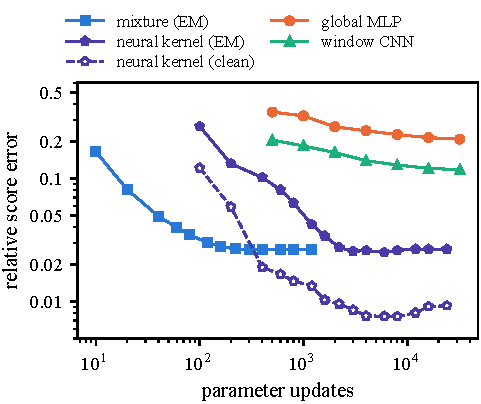
\includegraphics{fig_steps}
  \caption{Step efficiency on the Laplace chain with $N=2048$: test score error against the number of parameter
  updates. One update is an EM iteration of the mixture, one Adam step of the neural kernel (ten per EM iteration), or
  one SGD step of a network. Median over 16 seeds.}
  \label{fig:steps}
  % src: tools/paper_figs/figs_v2.py::fig_steps on reports/core/e63_curves_wall.csv (E65 refits, frozen 4 Nov 2026)
\end{figure}

The kernels also need far fewer parameter updates (\cref{fig:steps}). With 2{,}048 sequences the mixture passes the
final error of the window CNN after 20 EM iterations and is close to its own best after about 160. The neural kernel
passes the CNN's final error after 400 Adam steps from noisy data, and after 200 from clean data. The CNN needs all
of its 32{,}000 steps to get there.
% src: fig_steps printout (medians, E65): em_bp below 0.1176 at 20, within 10% of its minimum at 160; energy x10 below
% 0.1176 at 400; clean energy x10 at 200; window final 0.1176 at 32,000
Fewer updates are not always less time, because each EM iteration runs BP over all the training sequences. From clean
data the neural kernel is also faster in wall-clock time than both networks; from noisy data the networks reach their
own, much higher, error first (\cref{app:compute}).
% src: e63_curves_wall.csv at N = 2048: clean kernel first vs window and MLP 16/16; noisy kernel first 2/16

\subsection{When the data are not first-order Markov}
\label{sec:nonmarkov}

BP with a first-order kernel assumes first-order Markov data. When the data are not, the advantage over the networks
shrinks with the distance between the data and the closest first-order chain, and the networks win once this distance
is above about $10^{-2}$ nats per site (\cref{app:nonmarkov}). For a second-order chain there is a simple fix: pairs of
neighbouring sites form a first-order chain again, so BP on pairs is exact, and EM on pairs brings the advantage back.
% src: thesis exp_21_clean + E62: break-even delta 1-4e-2; E62 pair state below the best network >= 7/8 at every phi2

\section{Application: the stochastic Allen--Cahn field}
\label{sec:allen-cahn}

The stochastic Allen--Cahn equation \cite{allen1979microscopic,dapratozabczyk2014} describes a field that relaxes in a
double-well potential $V(\phi)=\tfrac14(\phi^2-1)^2$ while being shaken by heat,
\begin{equation}
  \partial_\tau\phi=\partial_x^2\phi-V'(\phi)+\sqrt{2\Theta}\,\eta,
\end{equation}
with space-time white noise $\eta$ at temperature $\Theta$. On a lattice of spacing $h$ its stationary law is
\begin{equation}
  p(\boldsymbol\phi)\propto\exp\Big(-\frac1\Theta\sum_i\Big[\frac{(\phi_{i+1}-\phi_i)^2}{2h}+hV(\phi_i)\Big]\Big),
\end{equation}
which is exactly a nearest-neighbour chain, so everything above applies. What makes it harder than the Laplace chain is
that the \emph{shape} of the next value's law depends on the current value: between the two wells it is broad, inside a
well it is narrow and one-sided (\cref{app:field}). We use $\Theta=0.3$, where the field sits in one well or the other
with sharp jumps between them, chains of $L=32$ sites and $h=1$, for which neighbouring sites have correlation $0.85$, as
on the Laplace chain.
% src: outputs/E32/cells.json (rho1 = 0.848 at T0.3_h1)

\Cref{fig:results}b compares the same models. The mixture of \cref{sec:kernel-families} assumes the shift structure:
its mean moves linearly with the current value and its shape never changes. Its best member is close to a Gaussian
chain, and BP with a Gaussian kernel is linear, so it stays at the error of the best linear denoiser ($0.270$ against
$0.269$ with 2{,}048 sequences), from noisy and from clean data alike. The neural kernel has no such constraint and
learns the state-dependent law. From 2{,}048 noisy sequences its error is $0.033$, 2.6 times below the window CNN and
7.6 times below the MLP; from clean sequences it is ten times below the CNN. With very few sequences the CNN is the
better model: at $N=32$ it beats the neural kernel learned by EM in 5 of 8 seeds.
% src: E33 em_mixture raw 0.2705 (seeds 0-7), E58 mixture_clean 0.2693, lmmse 0.2692; E55 em_energy 0.0328; per-seed
% mean ratios window/energy 2.57, MLP/energy 7.63 (8/8 at N=2048, 3/8 at N=32); E58 energy_h16 vs window median ratio 10.7

\Cref{app:field} adds three higher temperatures and more kernels: every kernel whose shape can change with the current
value beats the best network trained on the same noisy data, and a kernel with the form of the lattice energy, with five
parameters, is the most accurate of all. A diffusion U-Net with $1.2\times10^{7}$ parameters, trained on the clean
sequences, needs four times more data than the neural kernel to reach the same error.
% src: figures/tab_field.tex; E55 finished cells (U-Net at N=8192 reaches the kernel's N=2048 error in every cell)

\section{Discussion}
\label{sec:discussion}

For Markov sequences, the structure a denoiser can use is not in the score, which diffusion makes non-local, but in the
posterior, which stays a tree. BP turns a kernel, a function of two numbers, into the exact score at every noise level,
and EM learns the kernel from noisy data with BP as its E-step, without differentiating through BP. A small neural
kernel removes the need to choose a family: it matches the Gaussian mixture where the mixture is right, and it stays
accurate where the mixture falls back to the linear denoiser.

\paragraph{What this suggests for diffusion models.} Learn the local law and infer globally. For data that are Markov
in some ordering, one learned kernel gives the score at every noise level, and a kernel learned on short sequences works
unchanged on long ones, at a cost linear in their length. For data that are not, a kernel could handle the Markov part
exactly and a network the rest.

\paragraph{Limits.} The Markov order has to be known: on pairs of sites a grid step costs $O(N_g^3)$ instead of
$O(N_g^2)$. Each site carries one number here; a state with $d$ numbers needs a grid of $N_g^d$ points. The graph must be
a tree, and the grid limits how small $t$ can be. Finally, a large network closes the gap when data are plentiful, so the
gain we measure is in data efficiency, which matters most where scientific data are scarce.

\paragraph{Related work.} EM with forward--backward as the E-step is the classical way to fit hidden Markov and
state-space models \cite{baum1970,rabiner1989tutorial,shumway1982em,cappe2005}, and grids for non-Gaussian filtering go
back to \cite{kitagawa1987}; here the hidden chain is the clean data, the emission is the diffusion noise, and the
fitted model is used for its score. Diffusion models can also be trained from corrupted data
\cite{daras2023ambient,rozet2024learning,bai2024em}, but they learn a network score. Analytic and structured denoisers
\cite{kamb2024analytic,kadkhodaie2024generalization}, belief propagation on hierarchical data
\cite{garnierbrun2024transformers,sclocchi2025phase,mei2024unets} and the statistical physics of diffusion
\cite{biroli2023generative,biroli2024dynamical,achilli2025memorization,bonnaire2025memorize,garnierbrun2026biased,garnierbrun2026foam}
ask what structure a denoiser exploits. Markov sequences are the simplest non-Gaussian case in which the exact denoiser
is computable and can be learned from noisy data alone.


\section*{Impact statement}
This paper studies how much a denoiser for diffusion models can gain from knowing that its data are Markov, on
synthetic sequences and a simulated physical field with known ground truth. We see no ethical concern specific to it.

\bibliography{references}
\bibliographystyle{icml2026}

\newpage
\appendix
\onecolumn
\section{The Gaussian and the Laplace chain}
\label{app:gaussian-laplace}

\paragraph{How non-local the Gaussian score gets.} \Cref{fig:locality-curve} follows the part of $\mathbf Q_t$ outside
the tridiagonal band as $t$ grows. It is zero at $t=0$, largest at $t^{*}\simeq0.075$, and it vanishes again at large
$t$, where $\mathbf Q_t$ tends to the identity. A denoiser that only sees a window of $r$ neighbours on each side cannot
reach the exact score even with unlimited data: its best relative error is $0.20$, $0.089$, $0.029$ and $0.0066$ for
$r=1$, 2, 4 and 8.
% src: thesis tools/fig_ch10.py::windowed_oracle([1,2,4,8]) = 0.2023, 0.0890, 0.0294, 0.0066 (alpha=0.85, L=32)

\begin{figure}[h]
  \centering
  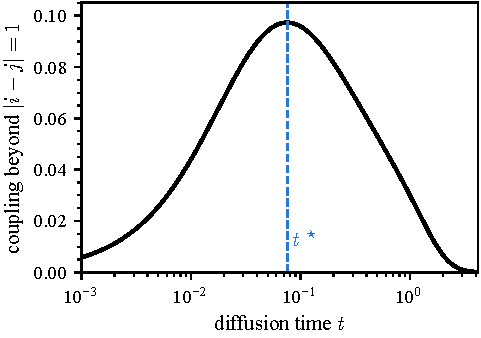
\includegraphics{fig_locality_curve}
  \caption{Size of $\mathbf Q_t$ outside the tridiagonal band, relative to the nearest-neighbour entries of
  $\mathbf Q_0$, against $t$ (Gaussian chain, $\alpha=0.85$, $L=24$). It peaks at $t^{*}\simeq0.075$.}
  \label{fig:locality-curve}
\end{figure}

\paragraph{The Laplace chain against the Gaussian chain.} The two chains have the same covariance; only the law of the
noise $\varepsilon_k$ differs (\cref{fig:laplace}a). The Laplace law has a sharp peak at zero and exponential tails.
\Cref{fig:laplace}b--c show the score of the middle site of a chain of nine, as its own noisy value changes and the
others stay at zero. At small noise the Laplace score saturates. A small deviation from the neighbours is treated as
noise and pulled back, more strongly than in the Gaussian chain ($-2.5$ against $-1.8$ at $x_k=0.5$, $t=0.05$). A large
one is believed, because the Laplace chain does make jumps, and only a bounded part of it is put down to noise ($-5.2$
against $-14.4$ at $x_k=4$). At large noise both scores are almost linear and almost equal. No linear denoiser can bend
like this, which is why the Gaussian approximation of \cref{fig:grid-vs-gaussian} fails at small noise.
% src: tools/paper_figs/thesis/fig_ch07.py grid_bp_score / gaussian_score (alpha=0.85, L=9, k=4), checked 8 Nov 2026

\begin{figure*}[h]
  \centering
  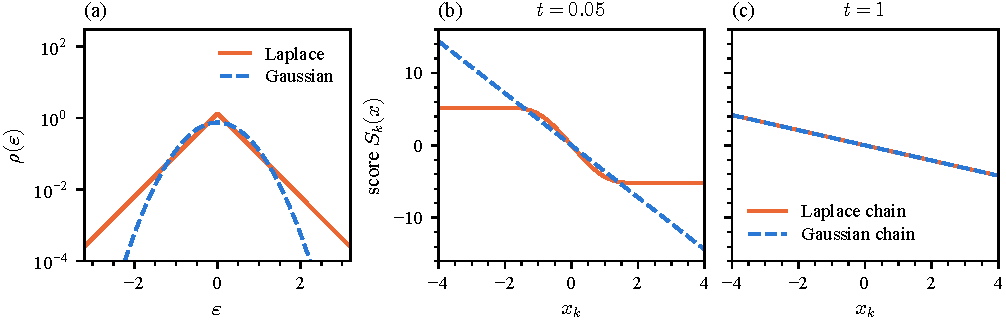
\includegraphics{fig_laplace}
  \caption{The Laplace chain. (a) Law of the noise $\varepsilon_k$, Laplace against Gaussian with the same variance.
  (b, c) Score of the middle site of a chain of nine against its own noisy value $x_k$, the other sites at zero, at
  $t=0.05$ and $t=1$. Exact scores from grid BP (Laplace) and in closed form (Gaussian).}
  \label{fig:laplace}
\end{figure*}

\section{Belief propagation on a grid}
\label{app:bp}

\paragraph{Recursions.} On the grid of \cref{sec:grid}, each column of the kernel matrix is normalised so that
$\sum_iw_iK_{ij}=1$, and $\mu$ is the law of the first site on the grid. The forward sweep is
\begin{equation}
  \tilde f_1=\mu\odot\ell_1,\qquad
  \tilde f_k=\ell_k\odot K\,(w\odot f_{k-1}),\qquad
  c_k=\sum_iw_i\tilde f_k(i),\qquad f_k=\tilde f_k/c_k ,
\end{equation}
and the backward sweep is
\begin{equation}
  b_L=\mathbf 1,\qquad
  \tilde b_k=K^{\top}\big(w\odot\ell_{k+1}\odot b_{k+1}\big),\qquad
  b_k=\tilde b_k\big/\textstyle\sum_iw_i\tilde b_k(i).
\end{equation}
The normalisations keep the numbers in floating-point range and do not change the result. The posterior mean of site
$k$ is the weighted average of the grid points with weights $w\odot f_k\odot b_k$. The pair posterior used by the E-step
is
\begin{equation}
  \xi_k(i,j)\propto f_k(j)\,w_j\,K_{ij}\,w_i\,\ell_{k+1}(i)\,b_{k+1}(i)
  \approx\Pr(a_k=g_j,\,a_{k+1}=g_i\mid\mathbf x),
\end{equation}
normalised to sum to one, and the log-likelihood of a sequence is $\log p(\mathbf x)=\sum_k\log c_k$, which comes for
free from the forward sweep.

\paragraph{Accuracy.} The grid spacing must resolve the noise term, whose width in $a$ is about $\sqrt{2t}$ at small $t$:
at $t=0.05$ it is $0.32$, eight times the spacing $h=0.04$. With $A=8$ the probability that falls outside the grid is
negligible. On the Gaussian chain, where the exact score is $-\mathbf Q_t\mathbf x$, grid BP reaches double-precision
round-off for $t\geq0.05$ already with 101 points (\cref{fig:grid}). On the Laplace chain we compare 401 with 801
points: over 2{,}000 sequences the scores differ by $1.1\times10^{-5}$ in relative terms at $t=0.05$, and by less at
larger $t$ (\cref{fig:grid-vs-gaussian}), at least a thousand times below every effect we report.
% src: fig_grid_gaussian (exp_01/grid_sweep_M.csv); figs_v2._closure_sweep (closure_sweep_2000.csv)

\begin{figure}[h]
  \centering
  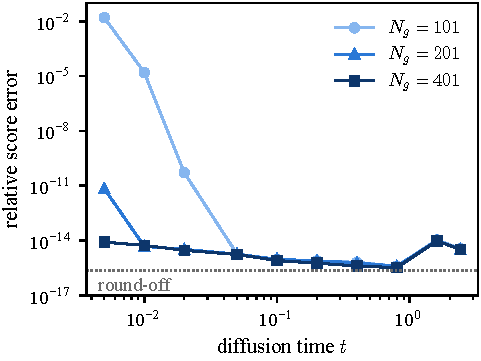
\includegraphics{fig_grid_gaussian}
  \caption{Grid BP against the exact score $-\mathbf Q_t\mathbf x$ of the Gaussian chain ($\alpha=0.8$) for three grid
  sizes. The dotted line is double-precision round-off.}
  \label{fig:grid}
\end{figure}

\section{Learning details}
\label{app:em}

\paragraph{Data and selection.} Each clean training sequence is noised once, at one of the twelve noise levels, so EM
sees $N$ noisy sequences in all. The networks instead see the clean sequences and draw fresh noise at every step. EM runs
up to 1{,}200 iterations (2{,}400 for the neural kernel) and keeps the kernel at fixed checkpoints; every model, kernel or
network, is tested at the checkpoint with the lowest score error on 1{,}024 validation sequences. Without the exact
score, EM can select by the likelihood of noisy validation sequences, which BP computes, and a network by its validation
loss: this changes the errors by at most $7\%$ and changes no ranking.
% src: experiments/e03_baselines.py::_one_view_groups; outputs/E02a/params_capacity.json; tools/core/read_e65.py (E65):
% free/oracle max em_bp 1.7%, spline 6.9%, energy 6.9%, networks <= 3.4%

\paragraph{M-steps.} For the mixture, the M-step is a closed-form update \cite{meng1993maximum}: each component's weight,
mean and variance are the weighted frequency, mean and variance of the residuals $g_i-\alpha g_j$, with weights $\Xi_{ij}$
times the component's responsibility, and $\alpha$ is then a weighted least-squares slope. For the Fourier kernel and
the other log-linear families, $Q$ is concave and its gradient is the observed minus the expected value of each basis
function, so a few gradient steps per iteration are enough. For the neural kernel, each M-step takes ten Adam steps on
$Q$, differentiating only through the network and its normalisation on the grid, and halves the step size whenever $Q$
does not increase, so the likelihood never decreases.

\paragraph{Stalled fits.} In our first implementation a rejected step kept Adam's memory, and 4 to 7\% of the neural
fits ended with a tiny step size, some of them close to their starting point. Restarting the optimiser after a rejected
step removes the problem. The results in the main text come from the first implementation; every fit, stalled or not,
enters the means quoted in the text, while the figures show medians, which a few stalled fits do not move.
% src: E58 outcome (23 of 576 fits), E55 finished cells (15 of 208 with final lr < 1e-10), E61 (0 of 448 after the fix)

\section{Training time}
\label{app:compute}

On one CPU thread at $N=2048$, an EM iteration takes $3.4$\,s for the mixture and $2.5$\,s for the neural kernel,
because BP runs over every training sequence; a clean-data iteration of the neural kernel takes $0.5$\,s. An SGD step
takes $2.5$\,ms for the window CNN and $1.0$\,ms for the MLP. \Cref{fig:wall} redraws \cref{fig:steps} against time.
From clean data the neural kernel reaches the final error of each network before the network does, in every seed. From
noisy data the networks are cheap per step and stop improving early, so they reach their own final error first, at five
to nine times the error of the kernels. At test time, BP on the 401-point grid takes about $7$\,ms per sequence for all
twelve noise levels.
% src: outputs/hpc_E63/timing.csv (E63, tools/core/read_e63.py D1); e63_curves_wall.csv at N = 2048

\begin{figure}[h]
  \centering
  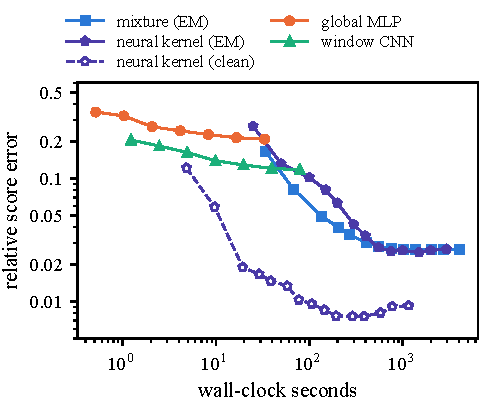
\includegraphics{fig_wall}
  \caption{The curves of \cref{fig:steps} against wall-clock seconds on one CPU thread ($N=2048$, median over 16
  seeds).}
  \label{fig:wall}
  % src: tools/paper_figs/figs_v2.py::fig_wall on reports/core/e63_curves_wall.csv
\end{figure}

\section{Other kernel families}
\label{app:families}

\paragraph{Shift families.} Besides the mixture, four families write the log-density of the noise as
\begin{equation}
  \log\varphi_\theta(\varepsilon)=-\frac{\lambda\varepsilon^2}{2}+\sum_{m=1}^{23}c_m\,b_m(\varepsilon)-\log Z_\theta,
\end{equation}
with the basis evaluated on $[-4,4]$ and held constant beyond it, where the quadratic term with learned $\lambda>0$ takes
over. With $\alpha$ and $\lambda$ each family has 25 parameters, like the mixture. The bases are cubic B-splines with
equally spaced knots, Gaussian bumps with equally spaced centres, a Fourier series ($\cos(m\pi\varepsilon/4)$ for
$m\le12$ and $\sin(m\pi\varepsilon/4)$ for $m\le11$) and Legendre polynomials. Splines and bumps are local and can
bend sharply at one point, as the Laplace peak requires; Fourier and Legendre are global and can only approximate it by
oscillating.

\paragraph{A kernel without the shift form.} The log-linear kernel writes $\log K_\theta(a'\mid a)$ in a $10\times10$
basis of B-splines in both arguments, 100 parameters, and is learned like the other log-linear families.

\paragraph{Results.} \Cref{fig:families} shows what each family learns, and \cref{fig:families-error} its error. The
four bases behave like the mixture: Fourier and Legendre oscillate in the tails, but the tails carry little
probability, and their errors are within 1.1 to 1.35 times that of the mixture. All five shift families beat the best
of six networks at every $N$ in every seed. The log-linear kernel learns slowly, because its 100 parameters are spread
over the whole plane, and it is the only kernel that loses to a network, the window CNN. The neural kernel is the
closest to the true kernel of all the families.
% src: tools/core/read_e56.py (E56): P1 16/16, P2 ratios 1.07-1.35, P4 loglinear2d vs window 0/16, P5 Hellinger
% energy 0.0394 (smallest), shift bases 0.046-0.049, loglinear2d 0.1071

\begin{figure*}[h]
  \centering
  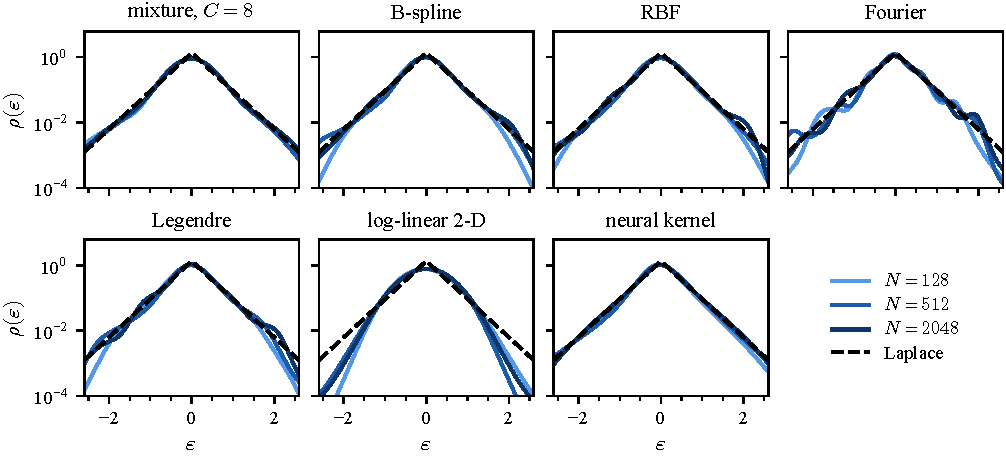
\includegraphics{fig_families}
  \caption{What each kernel family learns from noisy sequences: the learned law of the noise
  $\varepsilon=a_{k+1}-\alpha a_k$ from $N=128$, $512$ and $2048$ sequences, against the Laplace law (dashed). For the
  two families without the shift form we plot the learned $K(\varepsilon\mid a=0)$. One seed per $N$.}
  \label{fig:families}
  % src: mixture thesis exp_18 (innovation_density.csv); the six others outputs/hpc_E56_s*/densities.csv, seed 0
\end{figure*}

\begin{figure}[h]
  \centering
  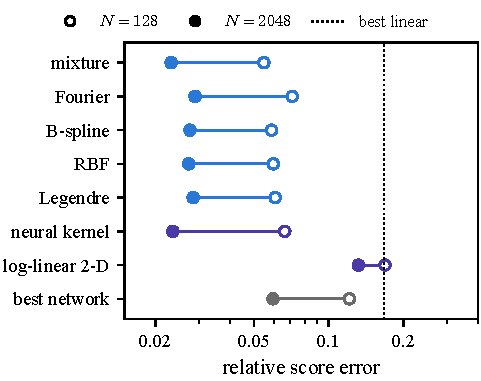
\includegraphics{fig_families_error}
  \caption{Relative score error of every kernel family learned by EM, and of the best of the six networks, from
  $N=128$ (open) and $N=2048$ (filled) sequences. Blue: families with the shift form; purple: families without it.
  Dotted: the best linear denoiser. Laplace chain, mean over 16 seeds, same test sequences.}
  \label{fig:families-error}
  % src: tools/paper_figs/figs_v2.py::fig_families_error (E02a em_bp, E56 kernels, E03 networks, E58 lmmse)
\end{figure}

\section{Other networks}
\label{app:networks}

\begin{table}[h]
  \caption{The six networks: the hyperparameters screened, the configuration kept, and its number of parameters. Every
  configuration kept predicts the noise.}
  \label{tab:networks}
  \centering
  \small
  \begin{tabular}{@{}llll r@{}}
    \toprule
    network & screened & kept & learning rate & parameters\\
    \midrule
    global MLP   & hidden $(128,128)$, $(256,256)$ & $(128,128)$ & $10^{-3}$ & 26{,}016\\
    window CNN   & radius $2,4,8$; width $64,128$ & radius 4, width 64 & $10^{-3}$ & 5{,}505\\
    TCN          & channels $32,64$; dilations $1,2,4,8$ & 32 channels & $10^{-3}$ & 17{,}057\\
    BiGRU        & hidden $32,64$ & 32 & $10^{-3}$ & 15{,}169\\
    transformer  & $(d,\text{heads},\text{layers})=(32,4,2),(64,4,2),(64,4,4)$ & $(32,4,2)$ & $3\times10^{-3}$ & 18{,}057\\
    U-Net        & channels $16,32$ & 16 & $10^{-3}$ & 13{,}713\\
    \bottomrule
  \end{tabular}
  % src: outputs/E03/params_confirm.json (grids), outputs/E03/winners.json, outputs/E03/confirm.csv (n_params)
\end{table}

\paragraph{Training.} Denoising score matching on the clean training sequences: each example gets a noise level drawn
from the twelve and fresh noise at every step; batch 64, Adam, gradient clipping at 1, 32{,}000 steps. For each
architecture, the grid of \cref{tab:networks}, two learning rates and two output parameterisations were screened on
four separate seeds, and the best configuration was kept for every $N$. Kernels and networks are tested on exactly the
same sequences.
% src: outputs/E03/params_confirm.json; tools/paper_figs/make_paper_figures.py::_paired_e03

\paragraph{Results.} \Cref{fig:networks} puts the six networks on one plot with the two kernels learned by EM. The
global MLP is the worst at every $N$, and the window CNN stops improving at about $0.12$. The four sequence models keep
improving with $N$, and BiGRU is the best network from $N=128$ on, still 2.2 to 2.8 times worse than the mixture. The
neural kernel beats each of the six networks in every seed at every $N$, with one exception (BiGRU at $N=512$, 15 of 16
seeds).
% src: per-seed mean ratios (E03 vs E02a): BiGRU 2.22, 2.45, 2.24, 2.83; read_e56 paired wins energy vs each network

\begin{figure}[h]
  \centering
  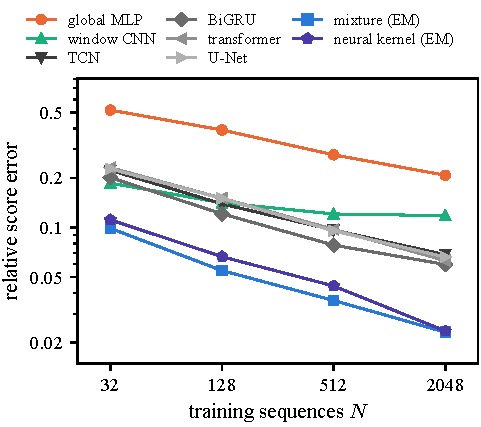
\includegraphics{fig_networks}
  \caption{The six networks against the mixture and the neural kernel learned by EM. Laplace chain, mean over 16 seeds,
  same test sequences.}
  \label{fig:networks}
  % src: E02a em_bp, E56 energy, E03 confirm.csv (tools/paper_figs/figs_v2.py::fig_networks)
\end{figure}

\paragraph{The model or the objective?} To separate the two, we also trained the neural kernel with the networks' own
recipe: denoising score matching on the clean sequences, with the posterior mean computed by a differentiable version
of BP \cite{eisner2016}. Trained this way it still beats the best of the six networks in every seed at every $N$
($0.018$ against $0.060$ for BiGRU at $N=2048$), so the gain comes from the model. Maximum likelihood on the same clean
sequences is better still, by a factor 1.3 to 2.5.
% src: tools/core/read_e66.py (E66): P1 16/16 every N, 0.0183 vs BiGRU 0.0596 at N=2048; ratio to E58 clean ML 1.31-2.46

\section{Data that are not first-order Markov}
\label{app:nonmarkov}

\paragraph{Three ways to break the assumption.} (i) A global latent variable: one Gaussian number per sequence is added
to every site of a Gaussian or Laplace chain, at four strengths. (ii) Long-range couplings: the precision matrix of the
Gaussian chain gets extra entries between distant sites, at four strengths. (iii) Second-order chains:
$a_k=\phi_1a_{k-1}+\phi_2a_{k-2}+\varepsilon_k$ with Laplace noise, where $\phi_1$ is adjusted so that neighbouring
sites keep correlation $0.85$. In each case we measure how far the data are from first-order Markov by $\delta$, the
Kullback--Leibler divergence per site from the data to the closest first-order chain. First-order EM--BP, the global MLP
and the window CNN are trained on 2{,}048 sequences.
% src: archive/Diffusion/research/nongaussian-bp/outputs/frozen/exp_21_clean; experiments/registry/E62.json

\paragraph{One curve.} All the data sets fall on one curve (\cref{fig:nonmarkov-delta}). Close to Markov, at
$\delta\approx5\times10^{-6}$, the window CNN is 11 to 15 times worse than the first-order kernel and the MLP 18 to 22
times worse. The advantage shrinks steadily as $\delta$ grows, and the networks win beyond $\delta\approx1$ to
$4\times10^{-2}$ nats per site.
% src: fig_nonmarkov printout: beta=0.1 d=4.61e-6 cnn 14.84/10.92 mlp 22.48/17.64; break-even 1.08e-2 .. 3.96e-2

\begin{figure}[h]
  \centering
  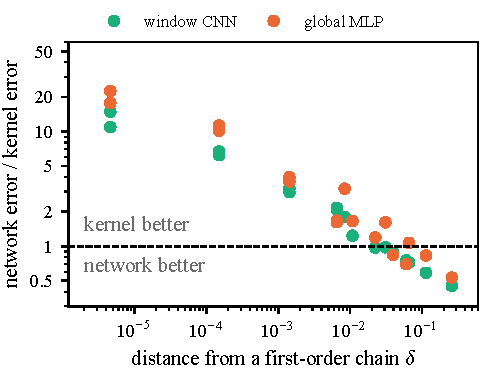
\includegraphics{fig_nonmarkov_delta}
  \caption{Error of a network divided by the error of first-order EM--BP, against the distance $\delta$ from the data to
  the closest first-order chain. Each point is one data set that is not first-order Markov (a global latent variable,
  long-range couplings, or a second-order chain, at increasing strength); $N=2048$. Above the dashed line the kernel
  is more accurate.}
  \label{fig:nonmarkov-delta}
  % src: thesis fig_ch10.py::_nonmarkov (frozen exp_21_clean), delta closed form; E62 via tools/core/read_e62.py
\end{figure}

\paragraph{Second-order chains.} Here the loss can be repaired. The first-order kernel's error grows with $\phi_2$ and
follows the exact error of the best possible first-order kernel, which we compute from the true chain
(\cref{fig:nonmarkov-ar2}): more data would not help, the model is wrong. Pairs of neighbouring sites $(a_{k-1},a_k)$,
however, form a first-order chain, so BP on pairs is exact, with a grid step that costs $O(N_g^3)$ instead of
$O(N_g^2)$. With a mixture kernel on pairs learned by the same EM, the error stays between $0.03$ and $0.04$ at every
$\phi_2$, below the best network in at least 7 of 8 seeds, and the learned $\phi_2$ is within $0.01$ of the truth.
% src: tools/core/read_e62.py (E62): P1 first/floor at 2048 = 1.01-1.13; P2 pair < first 8/8 (phi2 >= 0.1); P4 pair <
% best net >= 7/8 at every phi2 and N; D3 fitted phi2

\begin{figure}[h]
  \centering
  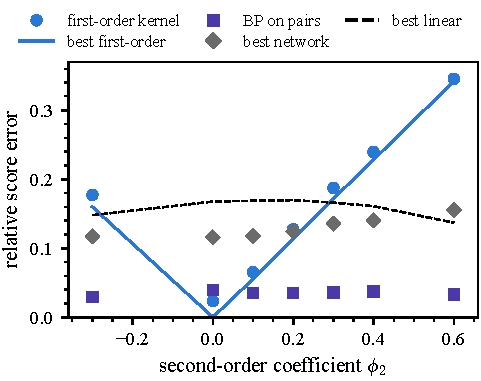
\includegraphics{fig_nonmarkov_ar2}
  \caption{Second-order Laplace chains, $N=2048$: the first-order kernel learned by EM, the best possible first-order
  kernel (line), the kernel on pairs of sites learned by EM, the best network, and the best linear denoiser. Mean over 8
  seeds.}
  \label{fig:nonmarkov-ar2}
  % src: E62 (frozen 6 Nov 2026), line = E62.json calibration_2026-11-02 first_order_floor
\end{figure}

\section{The Allen--Cahn field}
\label{app:field}

\paragraph{What the field looks like.} \Cref{fig:field} shows the chain of \cref{sec:allen-cahn}. The potential has two
wells at $\phi=\pm1$ (a). At $\Theta=0.3$ a sample sits in one well or the other and jumps between them; at $\Theta=2$
the heat dominates and the field looks like a Gaussian chain (b). The law of one site has two peaks at low temperature
and is close to Gaussian at high temperature (c). The exact kernel at $\Theta=0.3$ changes shape with the current value
$a$: broad between the wells, skewed towards the well from $a=0.6$, narrow and one-sided inside it (d). A shift family
can move the centre of $K(a'\mid a)$ with $a$, but not its shape. We work with the standardised field $a=\phi/s$, which
has unit variance, and choose the lattice spacing so that neighbouring sites have correlation $0.85$ at each
temperature.
% src: outputs/E32/cells.json (h = 1, 0.419, 0.226, 0.150 at Theta = 0.3, 0.5, 1, 2; rho1 0.848-0.850)

\begin{figure*}[h]
  \centering
  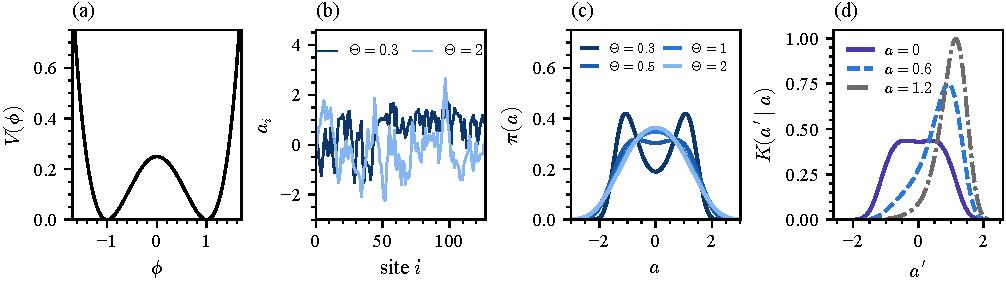
\includegraphics{fig_field}
  \caption{The Allen--Cahn field. (a) The double-well potential $V(\phi)$. (b) One exact sample of the standardised
  field at $\Theta=0.3$ and one at $\Theta=2$. (c) Law of one site at the four temperatures. (d) The exact kernel
  $K(a'\mid a)$ at $\Theta=0.3$ for three current values $a$.}
  \label{fig:field}
  % src: closed form and exact sampling (E32 cells), tools/paper_figs/figs_v2.py::fig_field
\end{figure*}

\paragraph{More kernels.} All are learned by EM through BP from noisy sequences. The \emph{site energy} (5 parameters)
has the form of the lattice energy, $K(a'\mid a)\propto\exp(-(a'-a)^2/2\gamma-f(a)-f(a'))$ with $f$ a polynomial of
degree four. The \emph{tilted spline} (25) is a random walk tilted by a learned function of $a'$. The \emph{free mixture}
(24) is a mixture of four Gaussians for the pair $(a,a')$, read as a conditional law. The \emph{log-linear} kernel
(100) and a \emph{mixture density network} (1{,}516) know nothing about the field. The neural kernel (337 to 1{,}185
parameters) and the shift mixture (25) are those of \cref{sec:kernel-families}. The networks of \cref{tab:field} are a
window CNN and a transformer, each trained in two ways on the same noisy sequences as EM, and we report the best of the
four; the U-Net is a diffusion U-Net with $1.2\times10^7$ parameters, trained on the clean sequences.

\paragraph{Results.} \Cref{tab:field} gives the errors relative to the best linear denoiser. Every kernel whose shape can
change with $a$ beats the best of the four networks at every temperature, including the ones that know nothing about
the field. The shift mixture is no better than the linear denoiser at any temperature. The site energy, which has the
right form, is the most accurate model everywhere. The U-Net is a much stronger network than the other four, and the
neural kernel still beats it in 30 of 32 paired seeds with 2{,}048 sequences; the U-Net needs 8{,}192 sequences to
reach the neural kernel's error.
% src: figures/tab_field.tex (tools/paper_figs/make_paper_figures.py::tab_field); E55 finished cells: wins 8/8/8/6;
% U-Net at N=8192 reaches the kernel's N=2048 error in every cell

\begin{table}[h]
  \caption{Allen--Cahn field: relative score error divided by that of the best linear denoiser, from 2{,}048 training
  sequences; mean over 16 seeds (8 for the neural kernel and the U-Net). Best of four: a window CNN and a transformer,
  each trained in two ways on the same noisy sequences as EM. Dashes: not run.}
  \label{tab:field}
  \centering
  \small
  \setlength{\tabcolsep}{3.5pt}
  \begin{tabular}{@{}lrcccc@{}}
\toprule
 & param. & $\Theta=0.3$ & $0.5$ & $1$ & $2$\\
\midrule
site energy & 5 & 0.033 & 0.072 & 0.141 & 0.169\\
neural kernel & 337--1{,}185 & 0.122 & 0.218 & 0.368 & 0.664\\
free mixture & 24 & 0.140 & 0.292 & 0.373 & 0.459\\
tilted spline & 25 & 0.060 & 0.134 & 0.280 & 0.428\\
log-linear 2-D & 100 & 0.184 & -- & 0.428 & --\\
MDN & 1{,}516 & 0.228 & 0.422 & 0.738 & 0.838\\
shift mixture & 25 & 1.004 & 1.004 & 1.014 & 1.021\\
\midrule
U-Net & $1.2\times10^{7}$ & 0.215 & 0.399 & 0.692 & 0.951\\
best of four &  & 0.484 & 1.174 & 2.157 & 3.044\\
\bottomrule
\end{tabular}

  % src: figures/tab_field.tex = tools/paper_figs/make_paper_figures.py::tab_field (E33, E43, E60, E55 finished cells)
\end{table}


\end{document}
